\question 下列关于临界区和临界资源叙述正确的是( )
\ding{192}.银行家算法可以用来解决临界区(Critical Section)问题
\ding{193}.一个正在访问临界资源的进程由于申请I/O操作而被阻塞时,不可以允许其他进程进入临界区和抢占处理机执行
\ding{194}.公用队列属于临界资源 \ding{195}.私用数据属于临界资源
\par\twoch{\ding{192}、\ding{193}}{\ding{192}、\ding{195}}{\textcolor{red}{只有\ding{194}}}{只有\ding{195}}
\begin{solution}临界资源是指每次仅允许一个进程访问的资源。每个进程中访问临界资源的那段代码称为临界区。
\ding{192}错误,银行家算法是避免死锁的算法。
\ding{193}错误,一个正在访问临界资源的进程由于申请I/O操作而被阻塞时,不允许其他进程进入临界区,但可以运行其他进程抢占处理机继续执行。
\ding{194}正确,公用队列可供多个进程使用,但一次只可有一个程序使用。
\ding{195}错误,私用数据仅供一个进程使用,不存在临界区问题。
因此,本题选择C选项。
\end{solution}
\question 进程A在执行过程中要使用临界资源,但要先获得进程B的计算结果,而此时进程B正在忙于I/O操作,则此时进程A应遵循同步机制应遵循的(
)准则
\par\twoch{\textcolor{red}{让权等待}}{空闲让进}{忙则等待}{有限等待}
\begin{solution}进程同步机制应遵循的4个准则为:空闲让进、忙则等待、有限等待和让权等待。其中每种准则的含义如下:

空闲让进。当没有进程处于临界区时,可以允许一个请求进入临界区的进程立即进入自己的临界区。
 忙则等待。当已有进程进入其临界区时,其他试图进入临界区的进程必须等待。

有限等待。对要求访问临界资源的进程,应保证能在有限的时间内进入自己的临界区。

让权等待。当一个进程因为某些原因不能进入自己的临界区时,应释放处理机给其他进程。
进程A需要进程B的结果,而此时进程B没法给A结果,因此A因为缺少数据而无法进入自己的临界区,应当遵循``让权等待''的准则,放弃处理机给其他进程,因此答案选择A选项。
\end{solution}
\question 关于临界问题的一个算法(假设只有进程P0和P1可能会进入临界区)如下(i为0或1代表进程P0或者P1):

~
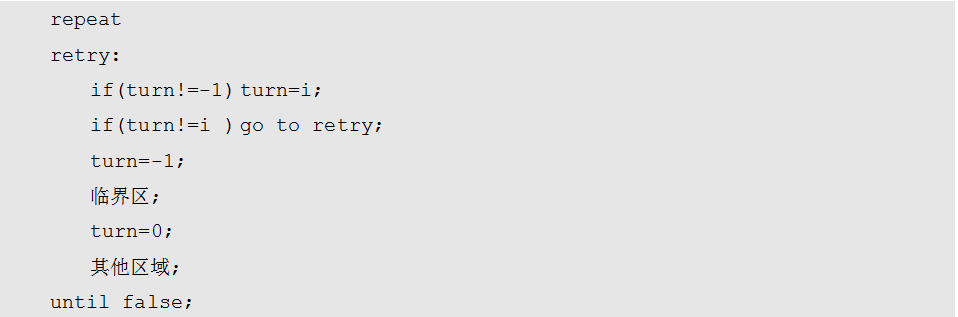
\includegraphics[width=2.42708in,height=0.80208in]{computerassets/00E4058A40E4544DAAE1BEED564B9DB8.png}

该算法( ~)
\par\fourch{不能保持进程互斥进入临界区,且会出现“饥饿”}{\textcolor{red}{不能保持进程互斥进入临界区,但不会出现“饥饿”}}{保证进程互斥进入临界区,但会出现“饥饿”}{保证进程互斥进入临界区,不会出现“饥饿”}
\begin{solution}进程并发时容易产生争夺资源现象,必须在入口码处阻止进程同时进入临界区。要求根据给出的入口码和出口码判断程序是否正确。此类出题方式较常见,关键是找出程序的错误。根据条件可先写出每个进程的执行代码,注意程序中i的取值应与进程Pi的取值相同:

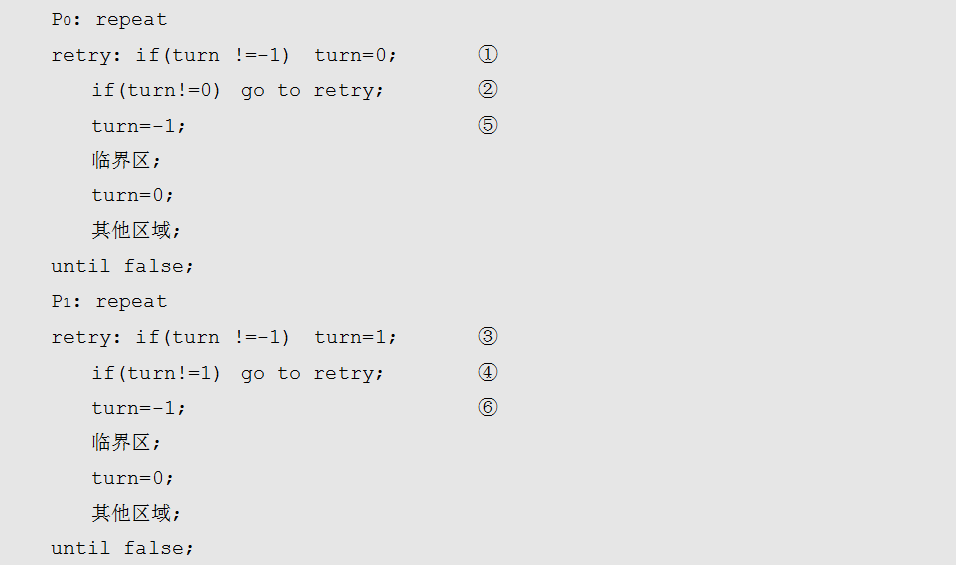
\includegraphics[width=2.42708in,height=1.43750in]{computerassets/16610B857D2D434ECA8B4A1A5391CCF1.png}

入口码最容易出错的地方就是在两个进程同时申请进入临界区的时候。若此时两个进程同时申请资源,此时turn的值是0,按照①②③④⑤⑥的顺序执行,两个进程同时进入临界区。再分析``饥饿''问题。因为入口码的判断条件是turn!=-1,否则进程被阻塞,而只有在有进程进入临界区的情况下turn的值才会是-1,所以没有进程会被饿死。
\end{solution}
\question 结构(Cobegin语句1;语句2 Coend)表示语句1和语句2并发执行。程序段如下:

~
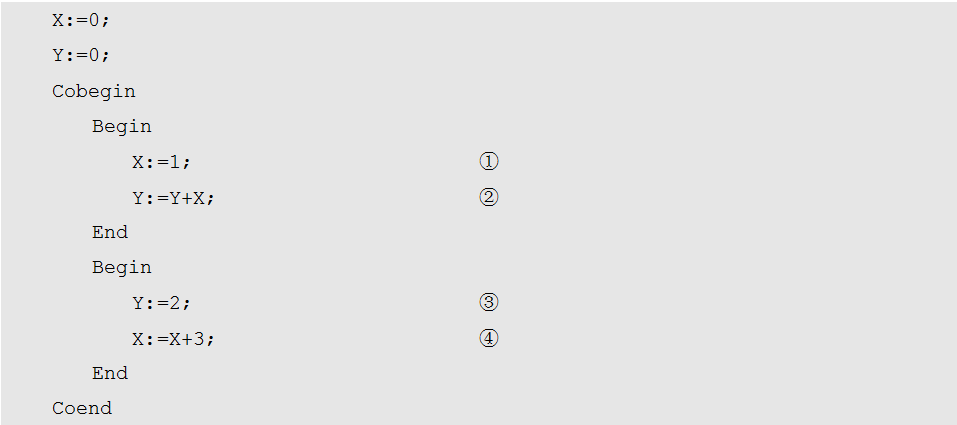
\includegraphics[width=2.42708in,height=1.07292in]{computerassets/4DDE49E225C2295AEB3F23EAC5BBDEF5.png}

当这个程序执行完时,变量X和Y的值有可能为( ~)。 \ding{192}.X=1,Y=2 \ding{193}.X=1,Y=3
\ding{194}.X=4,Y=6
\par\twoch{\ding{192}}{\ding{192}和\ding{193}}{\textcolor{red}{\ding{193}和\ding{194}}}{\ding{192}、\ding{193}和\ding{194}}
\begin{solution}由于语句并发执行,因此可能的执行顺序有①②③④(X=4,Y=2)、①③②④(X=4,Y=3)、①③④②(X=4,Y=6)、③④①②(X=1,Y=3),③①②④(X=4,Y=3)、③①④②(X=4,Y=6)这6种情况。所以应该选C。这类题主要考查对于并发执行的理解,列出所有可能情况时,注意Begin和End中的语句还是按顺序执行的。
\end{solution}
\question 进行p0和p1的共享变量定义及其初值为: boolean flag{[}2{]}; int turn=0;
flag{[}0{]}=FALSE; flag{[}1{]}=FALSE;
若进行p0和p1访问临界资源的类C代码实现如下: void p0() //进程p0 \{ while
(TRUE) \{ flag{[}0{]}=TRUE; turn=1; While (flag{[}1{]}\&\&(turn==1));
临界区; flag{[}0{]}=FALSE; \} \} void p1() //进程p1 \{ while (TRUE) \{
flag{[}1{]}=TRUE; turn=0; While (flag{[}0{]}\&\&(turn==0)); 临界区;
flag{[}1{]}=FALSE; \} \} 则并发执行进程p0和p1时产生的情形是( )
\par\fourch{不能保证进程互斥进入临界区,会出现“饥饿”现象}{不能保证进程互斥进入临界区,不会出现“饥饿”现象}{能保证进程互斥进入临界区,会出现“饥饿”现象}{\textcolor{red}{能保证进程互斥进入临界区,不会出现“饥饿”现象}}
\begin{solution}在之前没有了解过该算法的情况下,临场想要判断出来还是比较困难的,尤其本题的算法是一个可以保证进程互斥进入临界区且不会出现饥饿现象的良好算法,在考虑的时候,没法找出破绽,还容易误认为自己的想法不够全面而耽误时间。
下面分析算法。
首先是初始化步骤。第一步是初始化两个数组元素为FALSE,表明初始状态两个进程都没有打算进入临界区。第二步是turn置为0,这里的turn置为0并没有特殊的用意,有些读者会理解为优先执行进程P0,其实仔细分析并不是。因为对于turn的赋值操作都是在对turn的判断之前,也就是在程序执行开始后,都会先对turn值进行操作,然后才会判断,这里turn=0的用意仅仅是对turn值进行一个初始化,改为turn=1的效果也是完全相同的。
其次分析每个进程的执行流程(本题解释有些烦琐,如果已经掌握本题,跳过即可。对于不熟悉本题的读者,请紧跟解析,一次看完,中途打断思路可能会跟不上)。
由于进程P0和P1的执行流程类似,所以分析进程P0即可。假设此时进程P0要访问临界资源,进程P1尚未执行,开始执行题目中的代码,首先会进入第一个while循环(while(TRUE)),循环中第一行语句为``flag{[}0{]}=TRUE;
turn=1;'',将代表自己的flag置为TRUE,并将turn置为1,表明进程P0要申请访问临界资源(flag{[}0{]}=TRUE),并表明自己访问结束之后轮到进程P1访问临界资源(turn=1)。
接下来语句为``While
(flag{[}1{]}\&\&(turn==1));''。这句是很多考生粗心看错且很难弄明白含义的一个语句,本语句有着保证避免饥饿现象和互斥访问的作用,为本题的关键所在。
首先要注意这个while循环语句的最后有一个分号,表明该语句的含义是如果满足条件则执行空语句,直到不满足条件才跳出循环执行下面的语句,即不满足条件才进入临界区。在这一点上很多考生粗心漏看了分号而误认为本句是满足条件才进入临界区。
然后分析这句为什么能保证互斥访问和避免饥饿现象。先解释为什么能保证互斥。如果进程P1正在访问临界区,则相关变量的值为flag{[}0{]}=FALSE,flag{[}1{]}=TRUE,turn=0,这时候如果进程P0请求访问临界区,则会将flag{[}0{]}赋值为TRUE,turn赋值为1,此时相关变量就变为flag{[}0{]}=TRUE,flag{[}1{]}=TRUE,turn=1,此时进程P0会由于满足while循环的条件(flag{[}1{]}\&\&(turn==1))而不断执行空语句,直到进程P1访问完临界资源并将flag{[}1{]}置为FALSE,才能够跳出循环并进入临界区。对于进程P1情况类似,因此该算法能够保证两个进程互斥进入临界区。
接下来解释为什么能够避免饥饿现象。所谓饥饿现象是指某进程请求执行却长期得不到调度。本题中的一种饥饿现象就是进程P1提出申请,但系统却一直执行进程P0,导致进程P1长期得不到调度。分析相关变量情况。当进程P0正在临界区执行,此时进程P1提出进入临界区的请求时,执行``flag{[}1{]}=TRUE;
turn=0;''语句后,相关变量情况为flag{[}0{]}=TRUE,flag{[}1{]}=TRUE,turn=0。等待进程P0本次临界区执行结束(执行了flag{[}0{]}=FALSE;),紧接着进程P0又提出了访问请求,假设处理器总是优先执行进程P0的请求,则进程P0可以无阻碍地执行完``flag{[}0{]}=TRUE;
turn=1;'',此时相关变量情况为flag{[}0{]}=TRUE,flag{[}1{]}=TRUE,turn=1,则此时进程P0会执行语句``While
(flag{[}1{]}
\&\&(turn==1));''。这时候会由于满足条件而不断执行空语句,由于仅仅依靠进程P0已经无法跳出循环(因为此时进程P0已经没有改变,flag{[}1{]}和turn的语句可以执行),这时进程P1也是执行对应的一条语句``While
(flag{[}0{]}\&\&(turn==0));'',由于turn=1,所以进程P1会跳出这个循环并进入临界区执行,因此在假设处理器非常偏心进程P0的情况下进程P1还是会得到执行。进程P1执行完之后,也会有类似情况而使进程P0得到调度执行,所以进程P0和进程P1是交替执行的,本算法并不存在饥饿现象。
实际上,该算法为Peterson算法,满足互斥、空闲让进、有限等待3条同步机制准则,可以达到比较好的同步效果。本算法通过flag数组保证两个进程互斥进入临界区,同时通过turn来保证两个进程交替执行,避免了饥饿现象。本算法的缺点是无法设置进程的优先级,比如不能做到在进程P1提出申请后,仍然使进程P0连续执行多次,只能交替执行。但瑕不掩瑜,这仍然是一个能选出正确选项的好算法。
\end{solution}
